\ylDisplay{Veerev pall} % Ülesande nimi
{Hans Daniel Kaimre} % Autor
{piirkonnavoor} % Voor
{2016} % Aasta
{G 8} % Ülesande nr.
{6} % Raskustase
{
% Teema: Dünaamika
\ifStatement
\begin{wrapfigure}{r}{0.3\textwidth}
	\vspace{-15pt}
	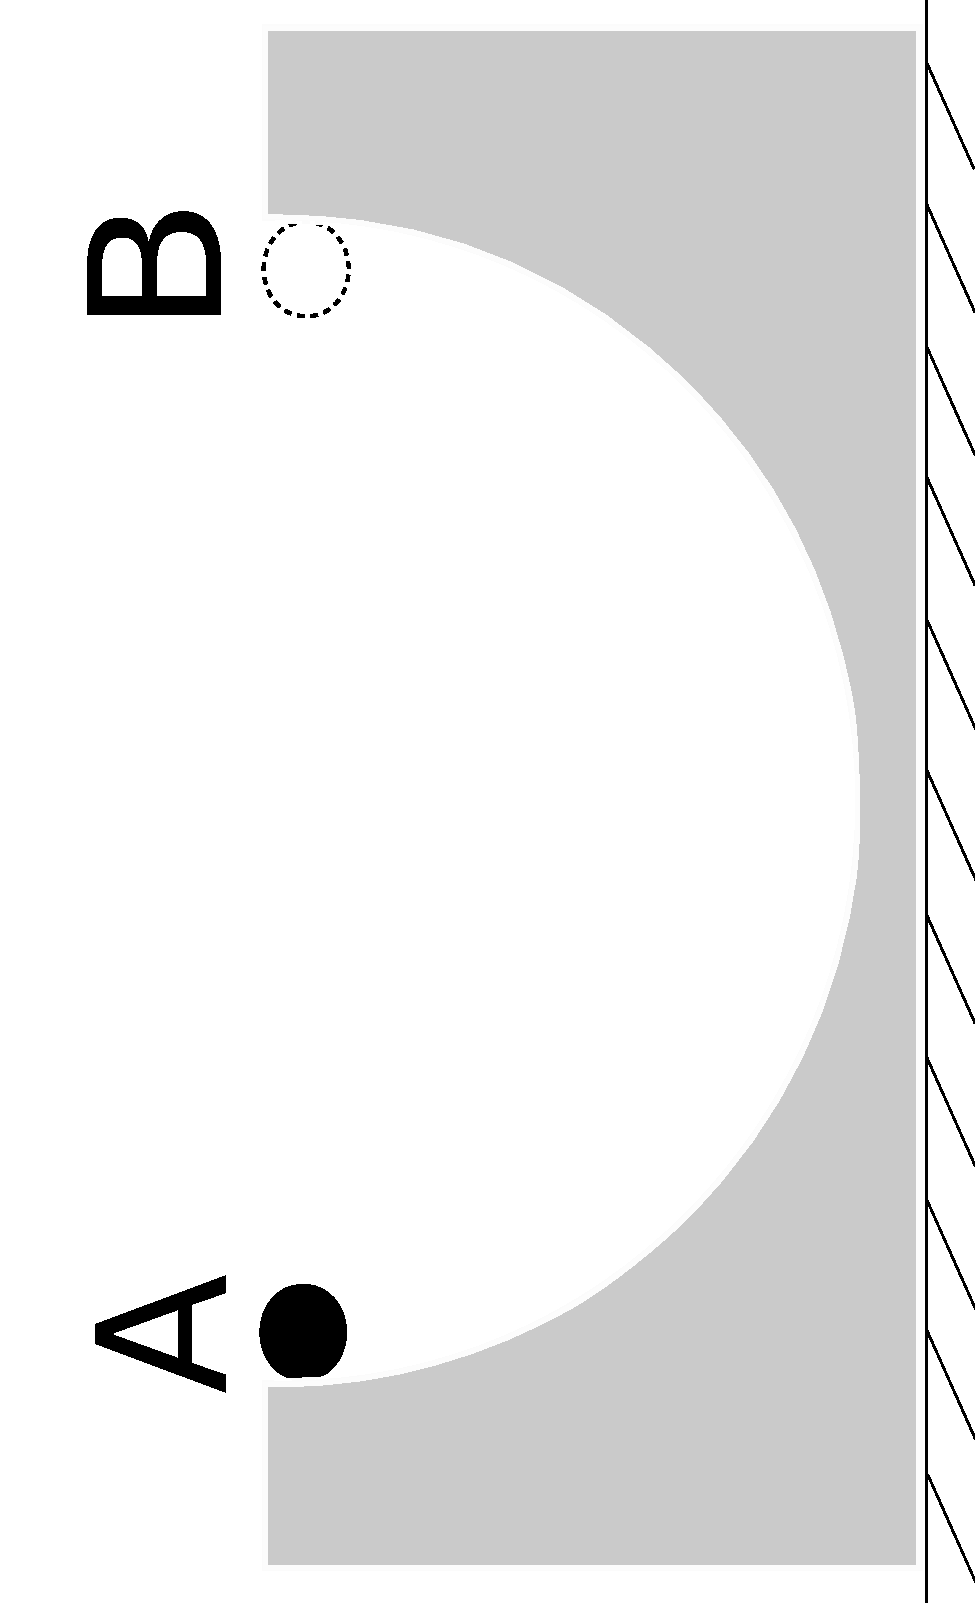
\includegraphics[angle=-90,origin=c,width=0.3\textwidth]{2016-v2g-08-halfpipe.pdf}
\end{wrapfigure}
Klotsist on välja lõigatud poolsilindrikujuline tükk raadiusega $R$. Klots seisab siledal hõõrdevabal horisontaalsel pinnal (vaata joonist). Klotsi mass on $M$. Punktist A lükatakse liikuma mööda silindrikujulise väljalõike pinda väike pall raadiusega $r$ ning massiga $m$. Kui palju on nihkunud klots hetkeks, mil pall jõuab punkti B?
\fi


\ifHint
Märkame, et kuna hõõrdejõud puudub, ei mõju süsteemile summaarset jõudu. Seega jääb klotsi ja palli summaarne massikese paigale.
\fi


\ifSolution
Olgu $x$-suunaline kiirus pallil $v_{x1}$ ning klotsil vastassuunas $v_{x2}$. Kuna hõõrdejõud pinnaga puudub, siis süsteemile horisontaalseid jõude ei mõju ja kehtib horisontaalse impulsi jäävuse seadus $mv_{x1}=Mv_{x2}$, kust $\frac{v_{x1}}{v_{x2}}=\frac{M}{m}$. Kuna see peab kehtima igal ajahetkel, siis järelikult kehtib ka $\frac{s_{x1}}{s_{x2}}=\frac{M}{m}$, kus $s_{x1}$ ja $s_{x2}$ on vastavalt palli ja aluse horisontaalsuunas läbitud vahemaad. Kui pall on jõudnud teise otsa, siis palli nihe klotsi suhtes on $2(R-r)$ (vahemaa palli keskmest punktis A palli keskmeni punktis B), seega $s_{x1}+s_{x2}=2(R-r)$. Avaldades $s_{x1} = s_{x2}\frac Mm$ ja asendades eelmisesse võrrandisse, saame 
$$s_{x2}=2(R-r)\frac{m}{M+m}.$$
\fi


\ifEngStatement
% Problem name: Rolling ball
\begin{wrapfigure}{r}{0.35\textwidth}
	\vspace{-10pt}
	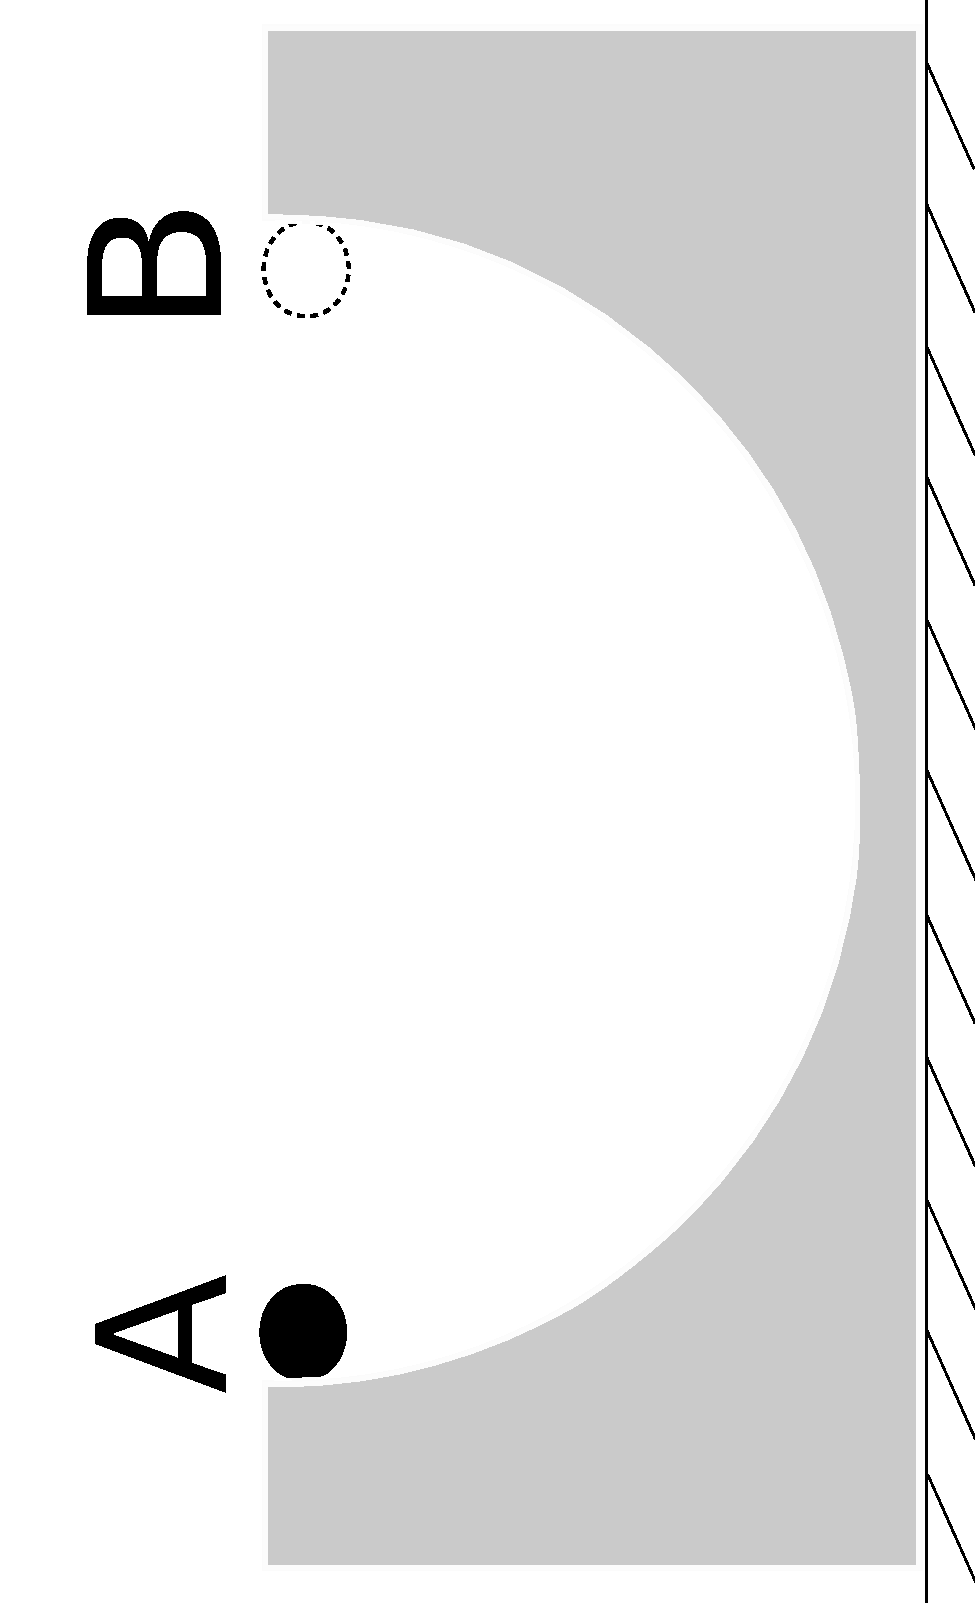
\includegraphics[angle=-90,origin=c,width=0.4\textwidth]{2016-v2g-08-halfpipe}
	\vspace{-60pt}
\end{wrapfigure}
A semi-cylindrical piece of radius $R$ is cut out from a tile. The tile is standing on a smooth frictionless horizontal surface (see figure). The tile’s mass is $M$. A small ball of radius $r$ and mass $m$ is pushed down from the point A to move along the cylindrical surface. How much has the tile moved by the moment when the ball reaches the point B?
\fi


\ifEngHint
Notice that because there is no friction force there is no total force applied to the system. Thus, the total center of mass of the ball and the tile stays still.
\fi


\ifEngSolution
Let the $x$-directional speed of the ball be $v_{x1}$ and for the tile $v_{x2}$ in the opposite direction. Because there is no friction with the surface no horizontal forces are applied to the system and the conservation of horizontal momentum applies: $mv_{x1}=Mv_{x2}$ where $\frac{v_{x1}}{v_{x2}}=\frac{M}{m}$. Because this must apply in each moment of time then therefore $\frac{s_{x1}}{s_{x2}}=\frac{M}{m}$ applies as well, where $s_{x1}$ and $s_{x2}$ are respectively the horizontal distances covered by the ball and the tile. If the ball has reached the other end then the ball’s displacement with respect to the tile is $2(R-r)$ (the distance between the ball’s center in the point A and the ball’s center in the point B), thus $s_{x1}+s_{x2}=2(R-r)$. Expressing $s_{x1} = s_{x2}\frac Mm$ and replacing it into the previous equation we get
$$s_{x2}=2(R-r)\frac{m}{M+m}.$$
\fi
}